\subsection{Genso}
GENSO is an abbreviation for Global Educational Network for Satellite Operations. As the name suggest GENSO is a network where satellite operators across the world can utilize each others ground stations. GENSO provides a stable network by the use of several Authentication Servers (AUS), that will synchronize with each other. This will make the network resistant to single point failures. As user of GENSO a software applications is available. This is the Ground Station Server (GSS). A GSS application allows Mission Control Clients (MCC) in the GENSO network to connect to the ground station and download data from space crafts. If the space craft is able, and local laws permit, it is also possible to upload data. Below is a figure illustrating this set up.   

\begin{figure}
\begin{center}
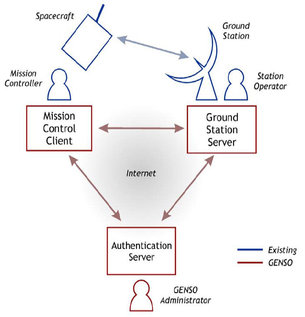
\includegraphics[width=1.0\textwidth]{/Figures/GENSO_network}
\end{center}
\caption{Illustration of the GENSO network.}
\label{GENSO_network}
\end{figure}

At first glance GENSO seems like a well organized ground station network which corresponds to the network we want to join. However it is difficult to find anything about the development of the project since September 2010. In addition the GENSO home page "GENSO.org" is not operational. Due to the difficulties with finding information of the current state of GENSO, we chose to look for other alternatives. 

Source: Educational part of ESAs' home page: http://www.esa.int/Education/Global_Educational_Network_for_Satellite_Operations 
    